\chapter{Pointingmodell}
Das Pointing von Teleskopen beschäftigt sich damit, dass das Teleskop so ausgerichtet wird, wie es erwünscht ist. Häufig ist das Problem, dass die eingestellte Position nicht exakt mit der gewünschten Position übereinstimmt. Gründe dafür können Fehler in der Präzision oder auch die Elastizität einzelner Bauteile sein. Da man die aufgenommen Daten mit den Bekannten Postionen am Himmel vergleichen kann, kann man versuchen ein Modell zu finden, welches die Fehler verkleinert oder im Idealfall sogar eliminiert.

\section{Koordinaten}
Das MST benutzt ein Koordinatensystem aus zwei Winkeln, welches den Kugelkoordinaten ähnelt. Der Azimutwinkel ($az$) beschreibt die Auslenkung in der Ebenen und läuft von $-180^{\circ}$ bis $180^{\circ}$, wobei es für $az=0^{\circ}$ in Richtung Norden ausgerichtet ist. Der Elevationswinkel $el$ läuft von $0^{\circ}$ bis $90^{\circ}$ wobei $el=90^{\circ}$ dem Zenit entspricht. Da es bei der Entwicklung von Pointingmodellen von Vorteil sein kann, in kartesischen Koordinaten zu rechnen, wird hier die Konvention verwendet, dass Nordrichtung der x-Richtung, die Westrichtung der y-Richtung und die Zenitrichtung der z-Richtung entspricht.
\begin{figure}[htbp]
\centering
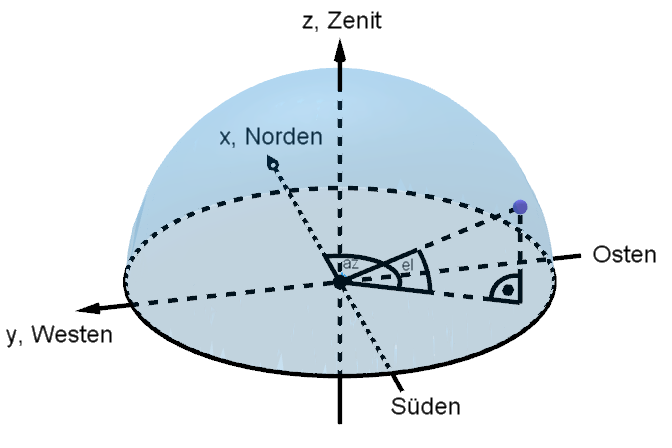
\includegraphics[width=0.7\textwidth]{Images/coordinates.png}
\caption{Die verwendeten Koordinaten}
\label{img:coordinates}
\end{figure}

\section{Entwicklung von Pointingmodellen}
Da man das Teleskop so ausrichten will, das die man die gewünschte Position vorgibt (Koordinaten der CCD- Index C) und dann die Koordinaten am Drive (Index D) einstellt, sucht man nach Funktionen, die die Koordinaten des Drives in Abhängigkeit von den gewünschten Koordinaten beschreibt. \\
\begin{equation}
az_D=f_{az}(az_C,el_C)
\end{equation}
\begin{equation}
el_D=f_{el}(az_C,el_C)
\label{eq:pointingprinciple}
\end{equation}
Ziel ist es, die Funktionen so zu optimieren, dass die Differenzen zu den gewünschten Koordinaten verschwinden.
\begin{equation}
\Delta_{az}=f_{az}(az_C,el_C)=0
\end{equation}
\begin{equation}
\Delta_{el}=f_{el}(az_C,el_C)=0
\label{eq:pointingZero}
\end{equation}

\section{Pointingmodell mit zwei Parametern}
\subsection{Vorhersage der CCD-Koordinaten in Abhängigkeit der Drive-Koordinaten}
Zunächst soll ein Pointingmodell mit zwei Parametern entwickelt werden, bei dem das Drivesystem in der Parkposition ($el_D=0,az_D=0$) in eine andere Richtung zeigt als die CCD-Kamera ($el_C=el_0,az_C=az_0$). Die beiden Positionen lassen sich auch durch zwei karthesische Richtungsvektoren $\vec{r_D}$ und $\vec{r_C}$ beschrieben. Ausgehend von dieser Startposition wird das Teleskop beziehungsweise die Vektoren $\vec{r_D}$ und $\vec{r_C}$ durch orthogonale Transformationen in die gewünschte Position gebracht wird. Als Parkpostion für das Drive-System erhält man mit den oben genannten Bedingung folgenden karthesischen Vektor:
\begin{equation}
\vec{r}_D^0=\left(\begin{array}{c} 1 \\ 0 \\ 0 \end{array}\right)
\label{eq:startDrive}
\end{equation}
Durch eine Drehung um die y-Achse mit dem Winkel $el$ und anschließender Drehung die z-Achse um den Winkel $az$ lässt sich aus dieser Startposition jeder Punkt auf der Einheitskugel erreichen. Die beiden Drehungen lassen sich zu einer Transformation $T(az,el)$ zusammenfassen:
\begin{equation}
T(az,el)=R_z(el)R_y(az)=
\left(\begin{array}{ccc} \cos(az) & \sin(el) & 0 \\ -\sin(el) & \cos(el) & 0 \\ 0 & 0 & 1\end{array}\right)
\left(\begin{array}{ccc} \cos(el) & 0 &-\sin(el) \\0 & 1 & 0\\ \sin(el) & 0 & \cos(el) \end{array} \right)
\end{equation}\\
\begin{equation}
T(az,el)=\left(\begin{array}{ccc} \cos(az)\cos(el) & \sin(az) &-\cos(az)\sin(el) \\-\cos(el)\sin(az) & \cos(az) & \sin(az)\sin(el)\\ \sin(el) & 0 & \cos(el) \end{array} \right)
\label{eq:TransformMat}
\end{equation}\\
Unter der Annahme, dass die Kamera von vornherein in eine andere Richtung als das Drive-System zeigt, lässt sich mit dieser Transformtion $T(az0,el0)$ aus der Startpostion des Drives die Startposition der Kamera bestimmen:
\begin{equation}
\vec{r}_C^0=T(az_0,el_0)\vec{r}_D^0=\left(\begin{array}{c} \cos(az_0)\cos(el_0) \\ -\cos(el_0)\sin(az_0) \\ \sin(el_0) \end{array}\right)
\label{eq:startCCD}
\end{equation}
Wendet man nun die gleiche Transformation $T(az_D,el_D)$ auf beide Startvektoren an, so erhält man für jedes Koordinatenpaar des Drives die zugehörigen Koordinaten der CCD in Abhängigkeit der Koordinaten des Drives. Für die Richtung des Drives ergibt sich
\begin{equation}
\vec{r}_D=T(az_D,el_D)\vec{r}_D^0=\left(\begin{array}{c} \cos(az)\cos(el) \\ -\cos(el)\sin(az) \\ \sin(el) \end{array}\right)
\label{eq:finDrive}
\end{equation}
und für die Richtung der CCD
\begin{equation}
\vec{r}_C=T(az,el)\vec{r}_C^0=\left(\begin{array}{c} \cos(az)\left(\cos(az_0)\cos(el)\cos(el_0)-\sin(el)\sin(el_0)\right)-\cos(el_0)\sin(az)\sin(az_0) \\
\sin(az)\left(\sin(el)\sin(el_0)-\cos(az_0)\cos(el)\cos(el_0)\right)-\cos(az)\cos(el_0)\sin(az_0) \\
\cos(az_0)\cos(el_0)\sin(el)+\cos(el)\sin(el_0) \end{array}\right)
\label{eq:finCCD}
\end{equation}
Aus diesen Richtungsvektoren müssen wieder die ursprünglichen Koordinaten $az$ und $el$ rekonstruiert werden. Die Elevation lässt sich aus der z-Komponente (Höhe) berechnen
\begin{equation}
el=\arcsin(r_z)
\label{eq:backtrafoEl}
\end{equation}
und der Azimutwinkel aus dem Verhältnis von y- zu x-Komponente. Da der Tangens dieses Verhaeltnis dem Azimuthwinkel mit einem Wertebereich von $-180^{\circ}$ bis $180^\circ$ entspricht muss man als Umkehrfunktion den erweiterten $\arctan$ vervewenden:
\begin{equation}
az=\arctan 2(r_y,r_x)=\left\{\begin{array}{lr}
\arctan\left(\frac{{r_y}}{{r_x}}\right) & r_x \textgreater 0  \\
\arctan\left(\frac{{r_y}}{{r_x}}\right)+\pi &  r_x \textless 0,r_y \textgreater 0 \\
\pm \pi   &  r_x \textless 0,r_y = 0 \\
\arctan\left(\frac{{r_y}}{{r_x}}\right)-\pi &  x \textless 0,r_y \textless 0 \\
+\frac{\pi}{2} &  x = 0,r_y \textgreater 0 \\
-\frac{\pi}{2} & x = 0,r_y \textless 0 \\
\end{array}
\label{eq:backtrafoAz}
\end{equation}

Somit lassen sich mit \ref{eq:backtrafoEl} beziehungsweise mit \ref{eq:backtrafoAz} in Verbindung mit \ref{eq:finCCD} die CCD-Koordinaten in Abhängigkeit der Drive-Koordinaten bestimmen:
\begin{equation}
el_C=\arcsin\left(\cos(az_0)\cos(el_0)\sin(el_D)+\sin(el_0)\cos(el_D)\right)
\label{eq:elD2C}
\end{equation}
\begin{equation}
az_C=\arctan2(
\sin(az_D)(\cos(el_D)\cos(az_0)\cos(el0)-\sin(el_D)\sin(el_0))-\cos(az_D)\sin(az_0)\cos(el0),
\cos(az_D)(\cos(el_D)\cos(az_0)\cos(el0)-\sin(el_D)\sin(el_0))+\sin(az_D)\sin(az_0)\cos(el0))
\label{eq:azD2C}
\end{equation}

\subsection{Vorhersage der Drive-Koordinaten in Abhängigkeit der CCD-Koordinaten}
Um die Abhängigkeiten der Drive-Koordinaten von den CCD-Koordinaten zu erhalten, muss das Gleichungssystem \ref{eq:elD2C} \ref{eq:azC2D} nach $el_D$ und $az_D$ aufgelöst werden. Da die Formel \ref{eq:elD2C} nur von $el_D$ und $el_C$ abhängt, kann diese unabhängig von \ref{eq:azC2D} umgestellt werden:

\begin{equation}
el_D=2\arctan\left(\frac{\cos(el_0)\cos(az_0)-\sqrt{\cos^2(el_0)\cos^2(az_0)-\sin^2(el_0)+\sin^2(el_C)}}{\sin(el_C)+\sin(el_0)}\right)
\label{eq:elC2D}
\end{equation}
Stellt man Gleichung \ref{eq:azC2D} nach $az_D$ um, so erhält man
\begin{equation}
az_D=(
\sin(az_C)(\cos(el_C)\cos(az_0)\cos(el0)-\sin(el_C)\sin(el_0))-\cos(az_C)\sin(az_0)\cos(el0),
\cos(az_C)(\cos(el_C)\cos(az_0)\cos(el0)-\sin(el_C)\sin(el_0))+\sin(az_C)\sin(az_0)\cos(el0))
\label{eq:azC2D}
\end{equation}
wobei hier noch $el_D$ durch den Ausdruck \ref{eq:elC2D} ersetzt werden muss.

\section{Erweiterung des Modells auf vier Parameter}
Unter der Annahme, dass die Skalen des Drivesystems einen Offset haben, also das der Wertebereich von $el_D$ beispielshalber von $1^{\circ}$ bis $91^{\circ}$ läuft kann das Modell mit zwei additiven Konstanten $el_1$ und $az_1$ erweitert werden. Das bedeutet, das bei der Vorhersage der CCD-Koordinaten \ref{eq:elD2C} und \ref{eq:azD2C} ein konstanter Offset zu den Argumenten hinzugefügt wird:
\begin{equation}
el_C^{4par}=el_C(el_D+el_1,az_D+az_1)
\label{eq:elD2C4}
\end{equation}
\begin{equation}
az_C^{4par}=az_C(el_D+el_1,az_D+az_1)
\label{eq:azD2C4}
\end{equation}
wohingegen bei der Vorhersage der Drive-Koordinaten nur ein konstanter Offset zu den Funktionen \ref{eq:elC2D} und \ref{eq:azC2D} addiert wird.
\begin{equation}
el_D^{4par}=el_D(el_C,az_C)+el_1
\label{eq:elD2C4}
\end{equation}
\begin{equation}
az_D^{4par}=az_D(el_C+,az_C)+az_1
\label{eq:azD2C4}
\end{equation}
